%%%% ijcai19.tex

\typeout{IJCAI-19 Instructions for Authors}

% These are the instructions for authors for IJCAI-19.

\documentclass{article}
\pdfpagewidth=8.5in
\pdfpageheight=11in
% The file ijcai19.sty is NOT the same than previous years'
\usepackage{ijcai19}

% Use the postscript times font!
\usepackage{times}
\usepackage{soul}
\usepackage{url}
\usepackage[hidelinks]{hyperref}
\usepackage[utf8]{inputenc}
\usepackage[small]{caption}
\usepackage{graphicx}
\usepackage{amsmath}
\usepackage{booktabs}
\usepackage{algorithm}
\usepackage{algorithmic}
% \usepackage{epstopdf}
\usepackage{makecell}
\usepackage{float}
\urlstyle{same}

% the following package is optional:
%\usepackage{latexsym}

% Following comment is from ijcai97-submit.tex:
% The preparation of these files was supported by Schlumberger Palo Alto
% Research, AT\&T Bell Laboratories, and Morgan Kaufmann Publishers.
% Shirley Jowell, of Morgan Kaufmann Publishers, and Peter F.
% Patel-Schneider, of AT\&T Bell Laboratories collaborated on their
% preparation.

% These instructions can be modified and used in other conferences as long
% as credit to the authors and supporting agencies is retained, this notice
% is not changed, and further modification or reuse is not restricted.
% Neither Shirley Jowell nor Peter F. Patel-Schneider can be listed as
% contacts for providing assistance without their prior permission.

% To use for other conferences, change references to files and the
% conference appropriate and use other authors, contacts, publishers, and
% organizations.
% Also change the deadline and address for returning papers and the length and
% page charge instructions.
% Put where the files are available in the appropriate places.

\title{Watercolor rendering and caustics effect for underwater scene} % TODO: TRANSLATE TO FRENCH MAYBE

% Multiple author syntax (remove the single-author syntax above and the \iffalse ... \fi here)
% Check the ijcai19-multiauthor.tex file for detailed instructions

\author{
Arnaud Paré-Vogt
\and
Mehdi Chaid
\affiliations
Département GIGL Polytechnique Montreal\\
\emails
arnaud.parevogt@gmail.com, % TODO: UPDATE WITH POLYMTL EMAIL
mehdi.chaid@polymtl.ca
}

\begin{document}

\maketitle

\begin{abstract}
TODO: Short summary about the project here.
\end{abstract}

\section{Introduction}

TODO: Talk about inspirations here. \medskip \par 

\noindent
TODO: Talk about the watercolor and caustics papers here.

% EXAMPLE HOW TO CITE HERE
% The first proof that shapes are fundamental in computer vision came from a very influential study on cognition, 
% by \cite{hubel1959receptive}, who described how biological neurons could extract features from images,
% amongst which certain types of neurons were activated specifically by edges. \medskip \par 

\newpage
\section{Scene}

\subsection{Framework}

TODO: Talk about learnopengl.com and the base framework here.

\subsection{Content}
The scene models an underwater environment. The floor is made of a square patch of sand, and multiple static low polygon meshes are scattered on it. In addition, an animated low polygon fish is placed in the water above. Only the sand model is textured, all other models use a constant color per face. Figure \ref{fig:scene_content} shows the models of the underwater scene without any effect applied on them.

\begin{figure}[h]
 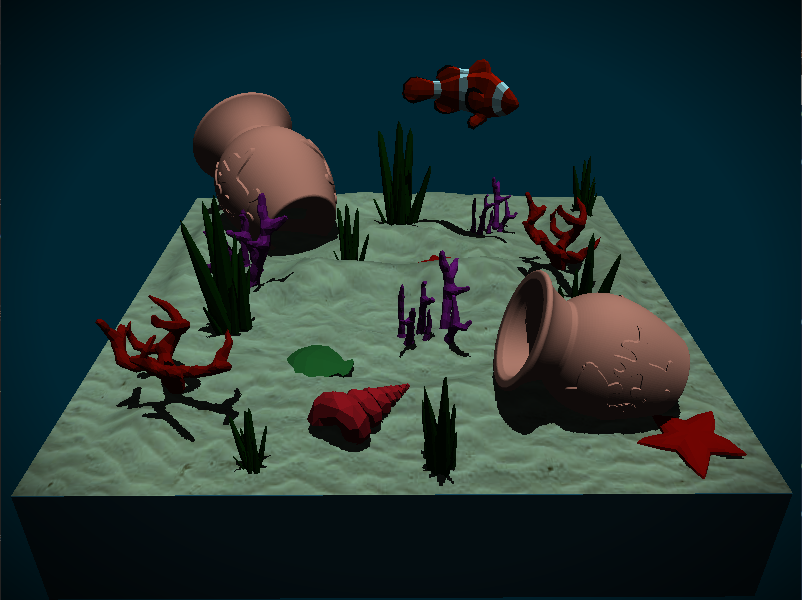
\includegraphics[width=\columnwidth]{imgs/scene_contents.png}
 \caption{content of the scene}
 \label{fig:scene_content}
\end{figure}

\subsection{Pipeline}

TODO: Talk about the shader pass pipeline here.

\newpage
\section{Watercolor rendering}

TODO: Talk about the watercolor rendering pipeline here.

\subsection{Cel shading}

TODO: Talk about cel shading here.

\subsection{Normal smoothing}

TODO: Talk about normal smoothing here.

\subsection{Morphological smoothing}

TODO: Talk about morphological smoothing here.

\subsection{Paper effects}

TODO: Talk about paper effects here.

\subsection{Edge darkening}

TODO: Talk about edge darkening here.

\subsection{Pigment density variation}

TODO: Talk about pigment density variation here.

\newpage
\section{Caustics}

In order to render caustics, we use a method called Periodic Caustic Textures \cite{periodic_caustic_textures}. This method is relatively simple. First, a grid with a certain resolution is generated. The grid is then rendered on a framebuffer. The vertex shader used in the rendering changes the x and y coordinates of the grid vertex by refracting the vertex as if it was a ray of light coming from above. The distorted mesh is then drawn in the fragment shader, using the ratio of the new area of a triangle over the original area of a triangle to calculate the color. This way, if the vertices are sent close together, the caustic color approaches white, while if the vertices are sent apart, the caustic color approaches black.

Figure \ref{fig:caustics_texture} shows the caustic texture generated by this approach.

\begin{figure}[h]
 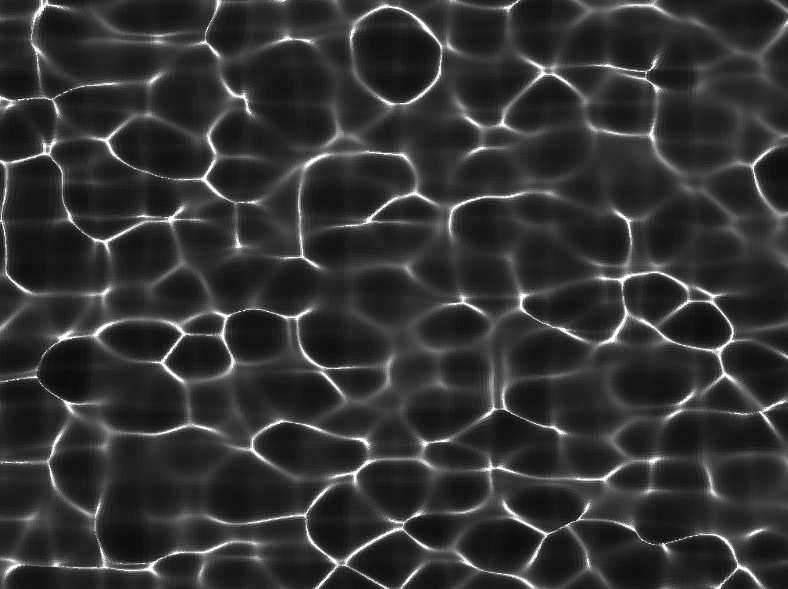
\includegraphics[width=\columnwidth]{imgs/caustics_texture.png}
 \caption{caustic texture generated from our implementation}
 \label{fig:caustics_texture}
\end{figure}

In order to generate this texture, we must be able to refract and project on the ground the grid vertices. This means that we need access to a water height and a water normal. We do this by generating fractal noise (in our case 3 layers of Perlin noise) to get the water height, and then we use the finite element difference method to compute the normal. All this work is done in the vertex shader. In order to generate the Perlin noise, an implementation from Stefan Gustavson was used \cite{perlin_noise}.

Once the caustic texture is generated, we project the texture on the scene to give the impression that the scene is illuminated by the caustics. This is an approximation, but the result is good enough. Figure \ref{fig:scene_with_caustics} shows the scene with the caustics projected on it.

\begin{figure}[h]
 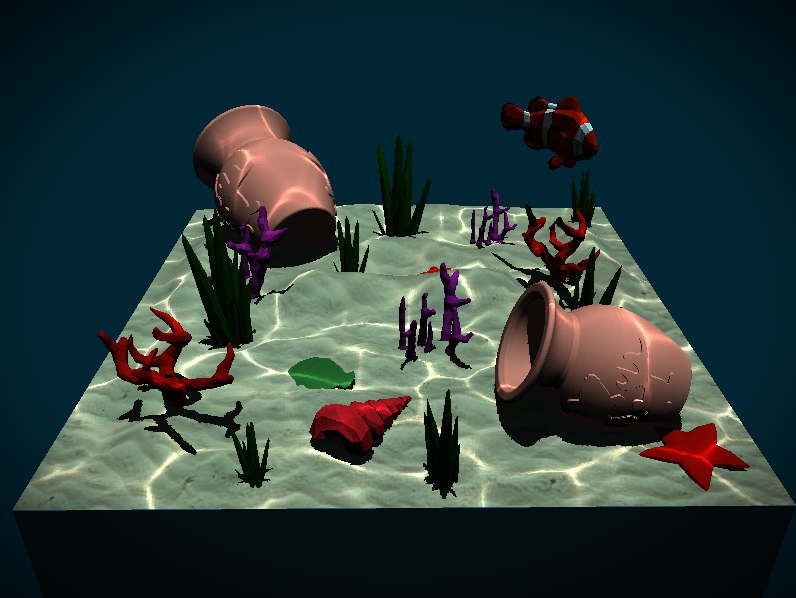
\includegraphics[width=\columnwidth]{imgs/scene_with_caustics.png}
 \caption{scene with the projected caustic texture}
 \label{fig:scene_with_caustics}
\end{figure}

\section{Underwater effects}

TODO: Talk about underwater effects here.

\section{Results}

TODO: Showcase more results here.

% \newpage
\section{Future Work}

TODO: Talk about possible improvements here.

\section{Conclusion}

TODO: Conclude here.

\newpage
\appendix

%% The file named.bst is a bibliography style file for BibTeX 0.99c
\bibliographystyle{named}
\bibliography{ijcai19}

% The reference section will autofill when we add \cite{} in the report.

\end{document}

